\documentclass[8pt]{beamer}
\usepackage{amsmath}
\usepackage[italian]{babel}
\usepackage{commath}
\usepackage[autostyle, english = american]{csquotes}
\usepackage{graphicx}
\usepackage{minted}
\usepackage{parskip}
\usepackage{subcaption}
%\usepackage{minted}
\usetheme{Boadilla}
\graphicspath{ {./} }
\begin{document}
\title{Esercitazione 3}
\subtitle{Ricerca della parola più lunga ed eliminazione di una riga}
\author{Corradini, De Luca, di Nuzzo, Frick, Ragazzini}
\institute{unibo}
\date{2019}
\setbeamercovered{transparent}
\begin{frame}
\titlepage
\end{frame}
\begin{frame}{Introduzione}
\LARGE
  L'esercitazione prevedeva la costruzione di due applicativi cliente/servitore che permettano rispettivamente di cancellare una riga da e di cercare la parola più lunga in un file.

  Per questa esercitazione sono stati usati due modelli di socket C: con e senza connessione.
  \normalsize
\end{frame}
\begin{frame}[fragile]{Parola più lunga - Servitore}
  
  Il servitore di ricerca della parola più lunga trova la parola più lunga in un file in seguito ad una richiesta del cliente.
  
  Per separare una parola dall'altra si serve di una tabella \texttt{is\_separator} 
  che viene preparata opportunamente all'avvio del programma.
  
  \begin{minted}{cpp}

if(!(pid = fork())) {
  buf[nReceived] = '\0';
  fd = open(buf, O_RDONLY);
  if(fd < 0) 	ris = -1;
  else {
  ris = 0; counter = 0;
  while (read(fd, &ch, sizeof(char))) {
    if (is_separator[ch]){ 
    if(counter > ris) ris = counter;
    counter = 0;
    } else counter++;
  }
  close(fd);
  }
}
  \end{minted}
  \normalsize

  %\textbf{Possibile ottimizzazione}: Nel caso le richieste siano molto più numerose delle modifiche ai file   sarebbe possibile ottimizzare il server pre-caricando la lunghezza della parola più lunga di ogni file, rispondendo quindi   alle richieste in tempo $O(1)$. Esempi di possibili applicazioni sono basi di dati di \textit{corpora}, nei quali i testi memorizzati   sul servitore vengono modificati molto raramente, dizionari e simili depositi di linguaggio naturale nei quali l'operazione di aggiornamento  più frequente è l'inserimento di nuovi file.
  
\end{frame}
\begin{frame}[fragile]{Parola più lunga - Cliente}
  Il cliente di ricerca della parola più lunga invia al proprio servitore le richieste di ricerca della parola più lunga in un file.
  
  I nomi dei file da analizzare sono letti all'interno di un ciclo \texttt{while (gets(nome\_file))}: 
  in questo modo, il programma termina con l'inserimento di EOF. 
  \small
  \begin{minted}{cpp}
while (gets(nome_file)) {
  printf("File da aprire: %s\n", nome_file);
  len = sizeof(servaddr);
  if(sendto(sd, nome_file, sizeof(char) * (strlen(nome_file) + 1), 0, (struct sockaddr *)&servaddr, len) < 0){
    perror("Errore: sendto non riuscita.\n"); continue;
  }
   printf("Attesa del risultato...\n");
  if (recvfrom(sd, &ris, sizeof(int), 0, (struct sockaddr *)&servaddr, &len) < 0){
    perror("Errore: recvfrom non riuscita.\n"); continue;
  }
  
  if(ris > 0) {
    printf("Esito dell'operazione: %d\n", ris);
  } else {
    printf("Errore: il file remoto non esiste.\n");
  }
  printf("Nome del file remoto, EOF per terminare: ");
}
  \end{minted}
\normalsize
\end{frame}
\begin{frame}[fragile]{Cancellazione righe - Servitore}
  Il servitore di cancellazione righe cancella una riga in un file in seguto ad una richiesta del cliente.

  Il servitore è protetto da attacchi di tipo \textit{buffer overflow}: 
  in caso di invio di una stringa troppo lunga legge solamente i primi 4 byte.

  \textbf{Assunto}: Per alleggerire il servitore i controlli di validità (esempio: positività del numero di riga, testualità del file in input) sono delegati al cliente:
  si presume quindi che tutti i dati ricevuti in input dalla socket siano validi. 

  \begin{minted}{cpp}
while (read(conn_sd, &buff, sizeof(buff)) > 0) {
  printf("%c", buff);
  if (currentLine != line)
  {
    write(conn_sd, &buff, sizeof(buff));
  }
  if (buff == '\n'){
    currentLine++;
    printf("DLS: Riga corrente %d\n", currentLine);
  }
}
  \end{minted}

  
\end{frame}
\begin{frame}[fragile]{Cancellazione righe - Cliente}
  Il cliente di cancellazione righe invia al proprio servitore le richieste di cancellazione di righe da un file.

  Nel caso il file non sia sufficientemente lungo per arrivare alla riga richiesta non viene mostrato alcun messaggio di errore, 
  né viene terminato il server. 
  \begin{minted}{cpp}
if ((pid = fork()) < 0) {
    printf("DLC: error on fork\n");
} else if (pid == 0) {
    while ((nread = read(ifd, fileRow, DIM_BUFF)) > 0) {
        write(sd, fileRow, nread);
    }
    shutdown(sd, 1);
} else if (pid > 0) {
    while ((nread = read(sd, fileRow, DIM_BUFF)) > 0) {
        write(ofd, fileRow, nread);
        write(1, fileRow, nread);
    }
    shutdown(sd, 0);
}
  \end{minted}
\end{frame}
\begin{frame}{Benchmark}
  \begin{columns}
    \begin{column}{0.45\textwidth}
  Il collo di bottiglia della ricerca della parola più lunga è la \textbf{lettura del file}.
  \begin{center}
    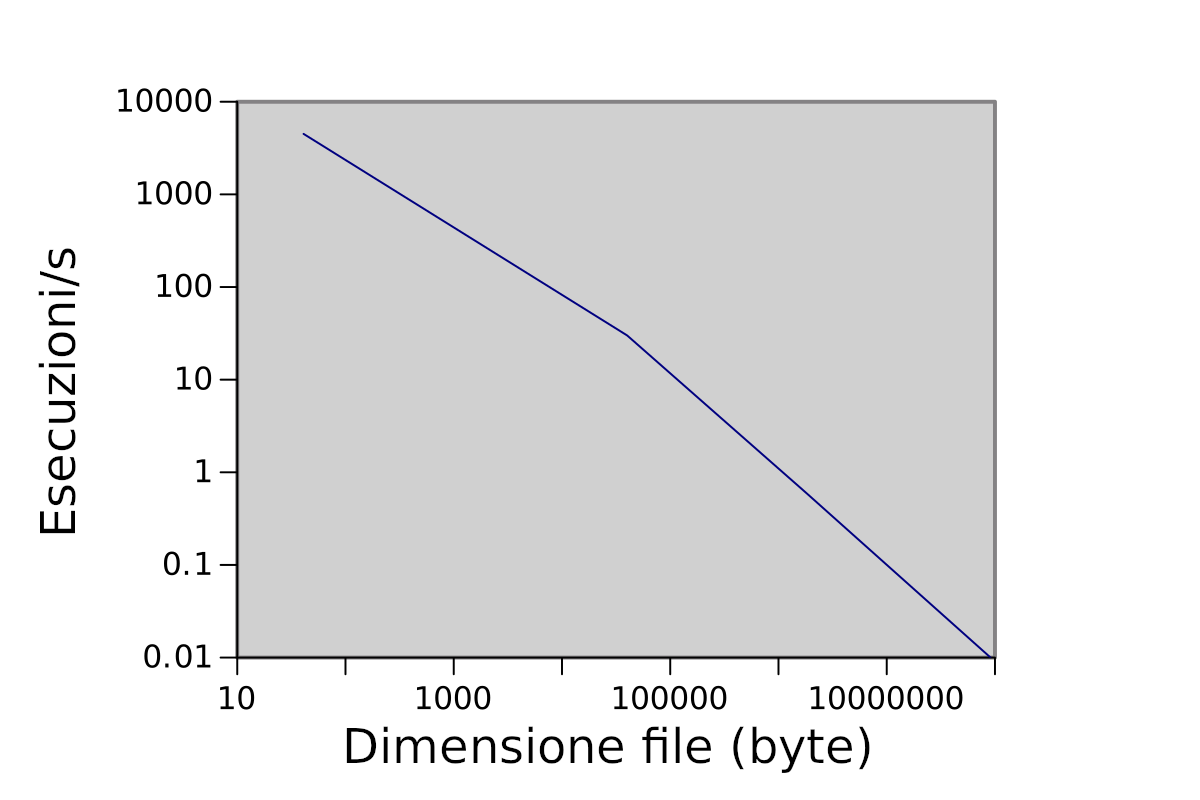
\includegraphics[width=\textwidth]{WLBench}
  \end{center}
\end{column}
\begin{column}{0.45\textwidth}
  Dovendo restituire l'intero file su \textit{standard input}, nell'eliminazione di una riga a questa si aggiunge l'\textbf{output del risultato}.
  \begin{center}
    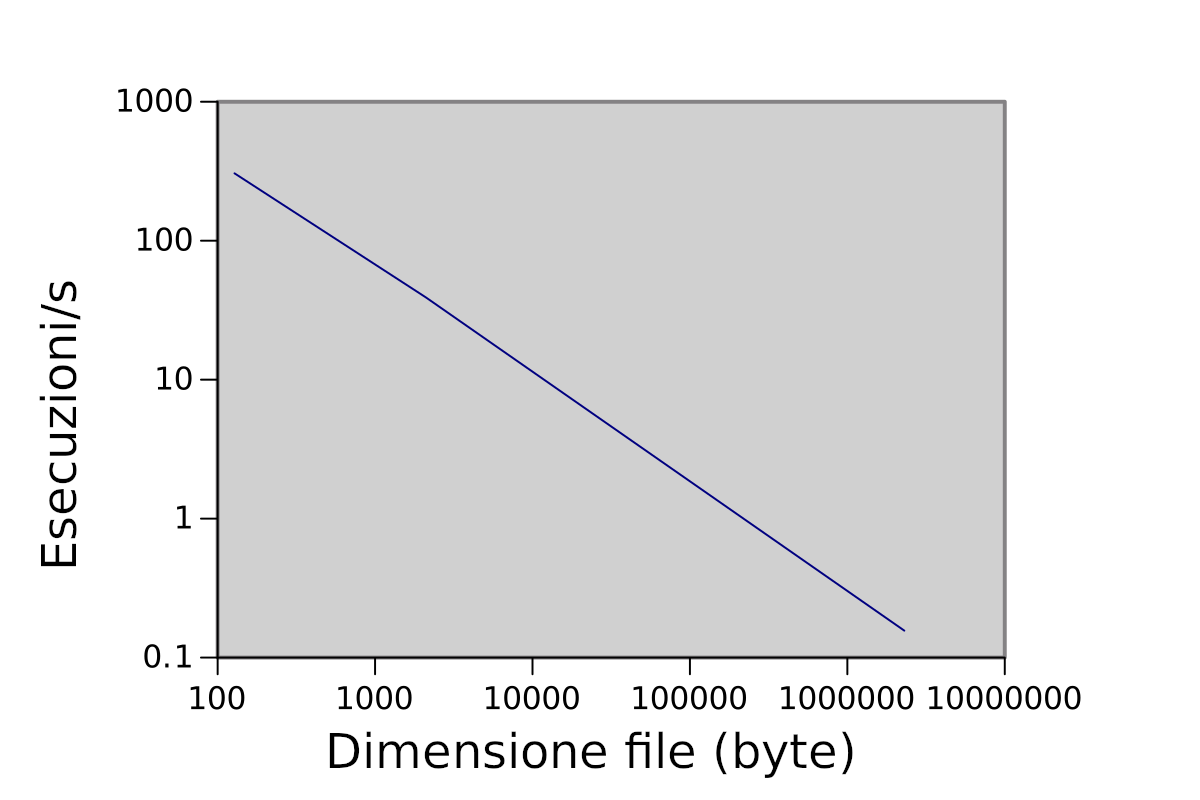
\includegraphics[width=\textwidth]{DLBench}
  \end{center}
\end{column}
\end{columns}
\end{frame}
\end{document}
